\section{\software}

\algoref{alg:UpdateNodePosition} describes the overview of \software. We first load all processed data from \secref{sec:{Data Description}} and apply VPSC \cite{dwyer2006fast} recursively to remove overlaps. We chose VPSC over other node overlap removal algorithms since VPSC is able to provide spread minimization and node movement minimization while maintaining a good level of global shape preservation \cite{chen2020Node}. During each recursion, we check node trajectories (See \algoref{alg:check river crossing}) and move back nodes that crossed a river. A recursion ends when 1) no overlaps are present; 2) no nodes crossed a river. We then increase the node size and repeat the recursion until the entire map canvas is filled.

% \begin{noindent}

\begin{algorithm}[tb!]
    \caption{The procedure to update node positions by removing overlaps and prevent nodes from crossing rivers.}\label{alg:UpdateNodePosition}
    \textbf{Variables:} \\
    $NodeList \gets$ a list of nodes representing CCGs \\
    $Node_{size}\gets$ the current size of all nodes \\
    $Node_{inc} \gets$ the increment node size of each iteration \\
    $Node_{max} \gets$ the maximum size of a node \\
    $Node_{stale} \gets$ the maximum number of iterations before a stalemate \\
    \begin{algorithmic}[1]
        \Procedure{UpdateNodePosition}{}
        \While{$ Node_{size} < Node_{max} $}

        \State $ nodeList_{ora} \gets $ RunVPSC ($ NodeList $)

            \For{$ node^i_{ora} \in nodeList_{ora} $}

                \If {MoveNode ($ Node^i, node^i_{ora} $)}
                    \State $ cross \gets $ \Call{CheckRiverCrossing}{$ Node^i, node^i_{ora} $}

                    \If{$ cross = True $}
                        \State $ Node^i.stale \gets Node^i.stale + 1 $

                        \If{$ Node^i.stale < Node_{stale} $}
                            \State \Call{MoveNode}{$ Node^i $}
                        \Else
                            \State \Call{DeriveCorridor}{$ Node^i, node^i_{ora} $}
                        \EndIf

                    \EndIf

                \EndIf

            \EndFor

        \EndWhile

        \State $Node_{size} \gets Node_{size} + Node_{inc}$

        \EndProcedure
    \end{algorithmic}
\end{algorithm}


\begin{algorithm}[tb!]
    \caption{The procedure to update a node's position.}\label{alg:move position}
    \begin{algorithmic}[1]
        \Procedure{MoveNode}{$ Node, Node_{new} $}
        \If{$ Node.x = Node_{new}.x $ and $ Node.y = Node_{new}.y $}
            \State \Return{$ False $}
        \EndIf
        
        \State init. $ x,y $

        \If{$ Node_{new}$ is $ undefined $}
            \State $previous \gets Node.history.pop() $
            \State $ x \gets previous.x,~y \gets previous.y $
        \Else
            \State $ x \gets Node_{new}.x,~y \gets Node_{new}.y $
            \State $ Node.history.push(x, y) $
        \EndIf

        \State $ Node.x \gets x $
        \State $ Node.y \gets y $
        \State \Return{$ True $}
        \EndProcedure
    \end{algorithmic}
\end{algorithm}

%\end{noindent}

\subsection{River Cross Checking}

We use rivers as topological boundaries to prevent nodes from crossing them. When a node's position changes, we check if the node's trajectory intersects any segment of a river, see \algoref{alg:check river crossing}. A boundary collision detection is performed to reduce the number of line intersection detections required.


% \begin{noindent}
\begin{algorithm}[tb!]
    \caption{The procedure to check if a node crosses a river.}\label{alg:check river crossing}
    \textbf{Variables:} \\
    $RiverEdges \gets$ a list of river edges formed by two points \\

    \begin{algorithmic}[1]
        \Procedure{CheckRiverCrossing}{$ Node, Node_{ora} $}
            \For{$ edge \in RiverEdges $}
                \State $ node_b \gets $ GenerateBoundary ($ Node, Node_{ora} $)
                \State $ edge_b \gets $ GenerateBoundary ($ edge $)
                \State $ collide \gets $ DetectBoundaryCollision ($ node_b, edge_b $)
                \If{$ collide = True $}
                    \State $ node_l \gets $ GenerateLine ($ Node, Node_{ora} $)
                    \State $ edge_l \gets $ GenerateLine ($ edge $)
                    \State $ intersect \gets $ DetectLineIntersection ($ node_l, edge_l $)
                    \If{$ intersect = True $}
                        \State \Return{$ True $}
                    \EndIf
                \EndIf
            \EndFor
            \State \Return{$ False $}
        \EndProcedure
    \end{algorithmic}
\end{algorithm}
%\end{noindent}

\subsection{Corridor Derivation}

As the VPSC always tries to produce an optimal node layout where node spread and movement are minimized, a node might be repeatedly traveling between two positions due to the lack of available space, creating a stalemate situation for recursions, as shown in \figref{fig:stalemate}. In order to create space for VPSC to generate a new layout, we introduce a user-adjustable parameter, $ Node_{stale} $, to break the stalemate: if a node is traveling between two positions for more than $ Node_{stale} $ iterations, it is considered to be in a stalemate. A stalemate triggers a corridor derivation which moves all nodes within the corridor by $ \mathcal{D} $ set by the user (See \figref{fig:corridor} and \algoref{alg:derive corridor}).

{
\begin{figure}[tb!]
    \centering
    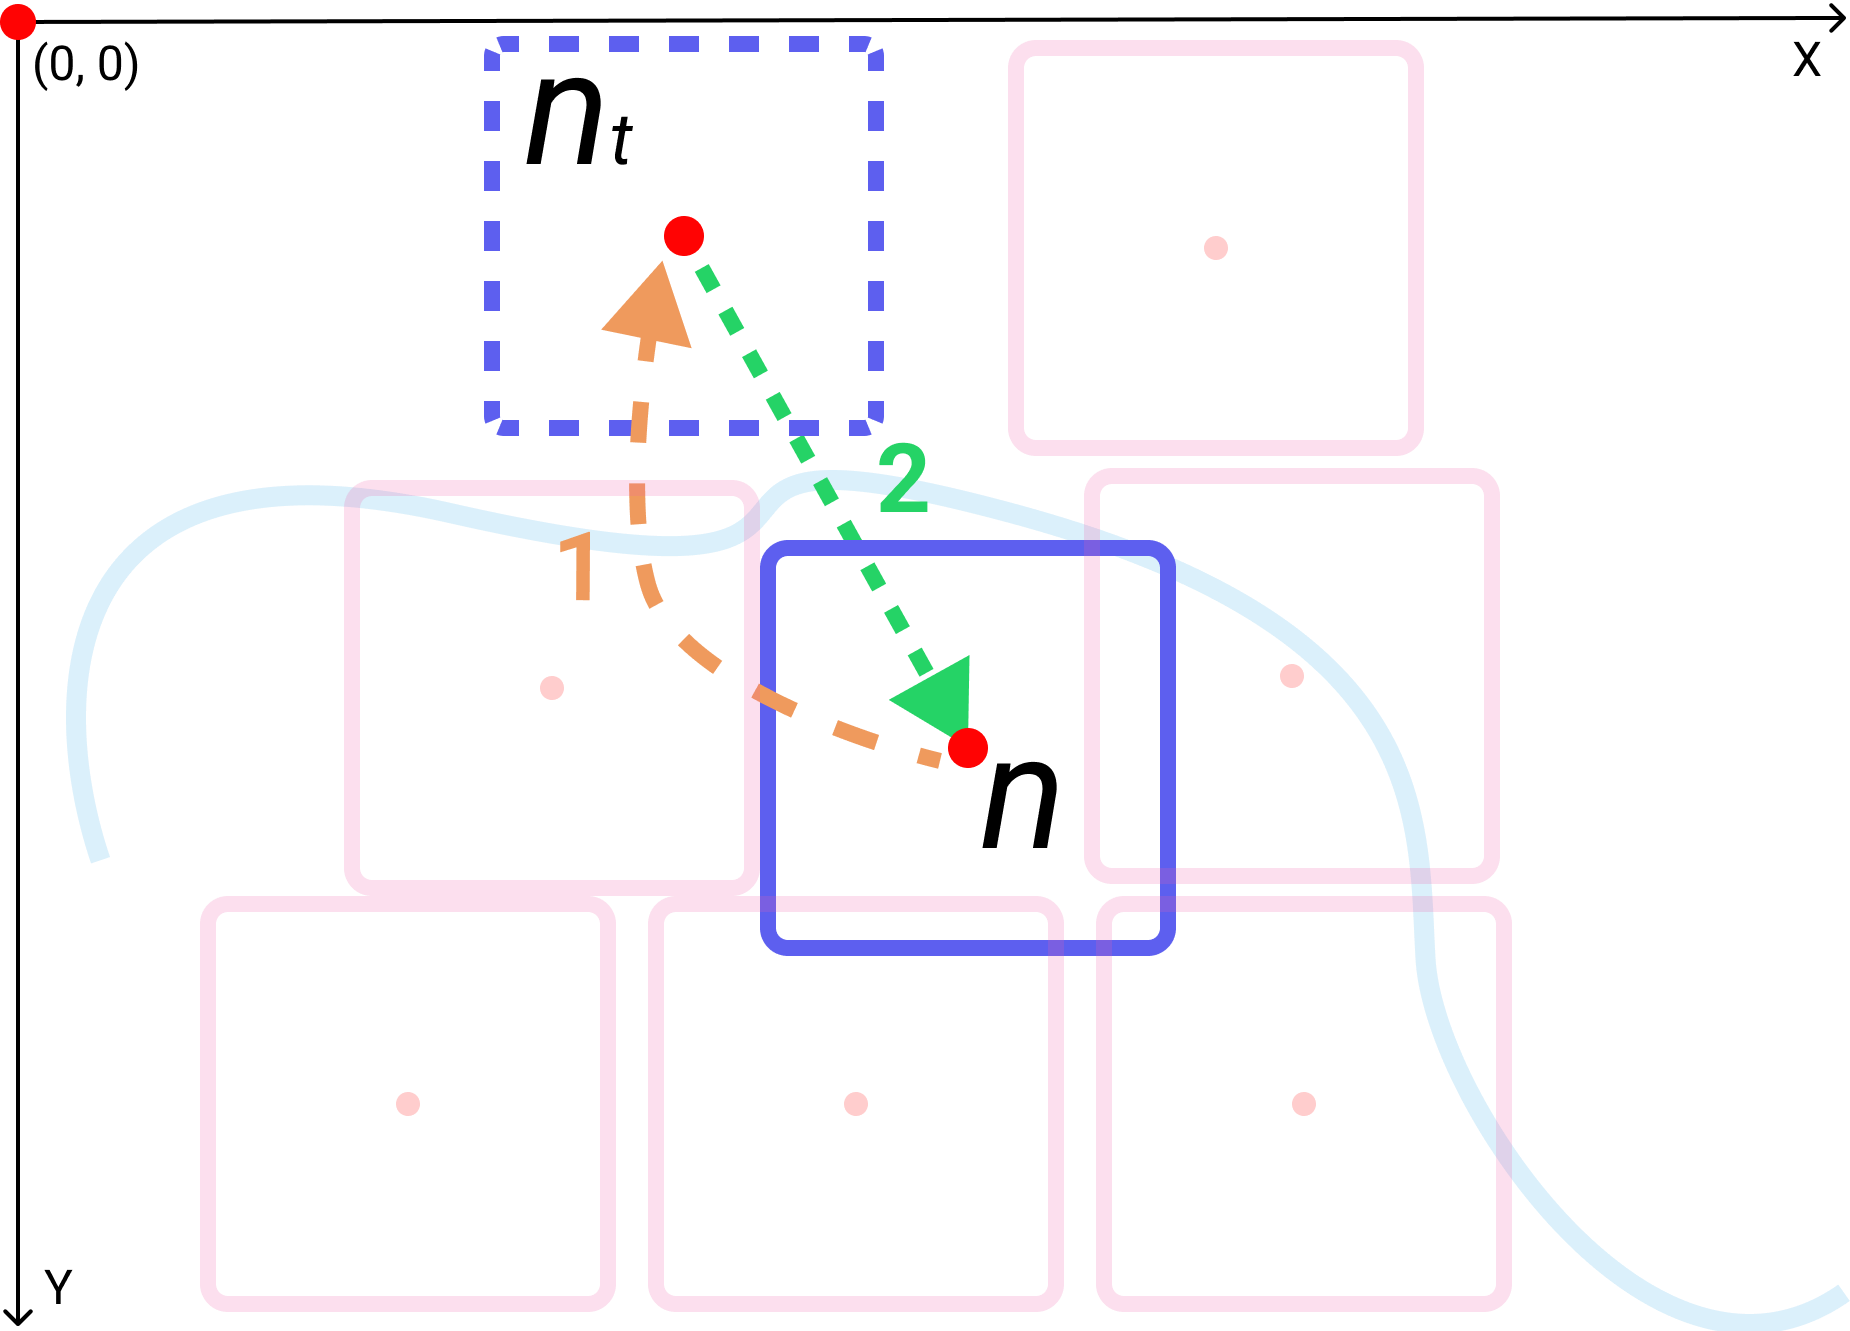
\includegraphics[width=\columnwidth]{figure/stalemate.png}
    \caption{A stalemate situation is when a node repeatedly travels between two positions (A and B) for more than $Node_{stale}$ iterations. }
    \label{fig:stalemate}
\end{figure}
}

{
\begin{figure}[tb!]
    \centering
    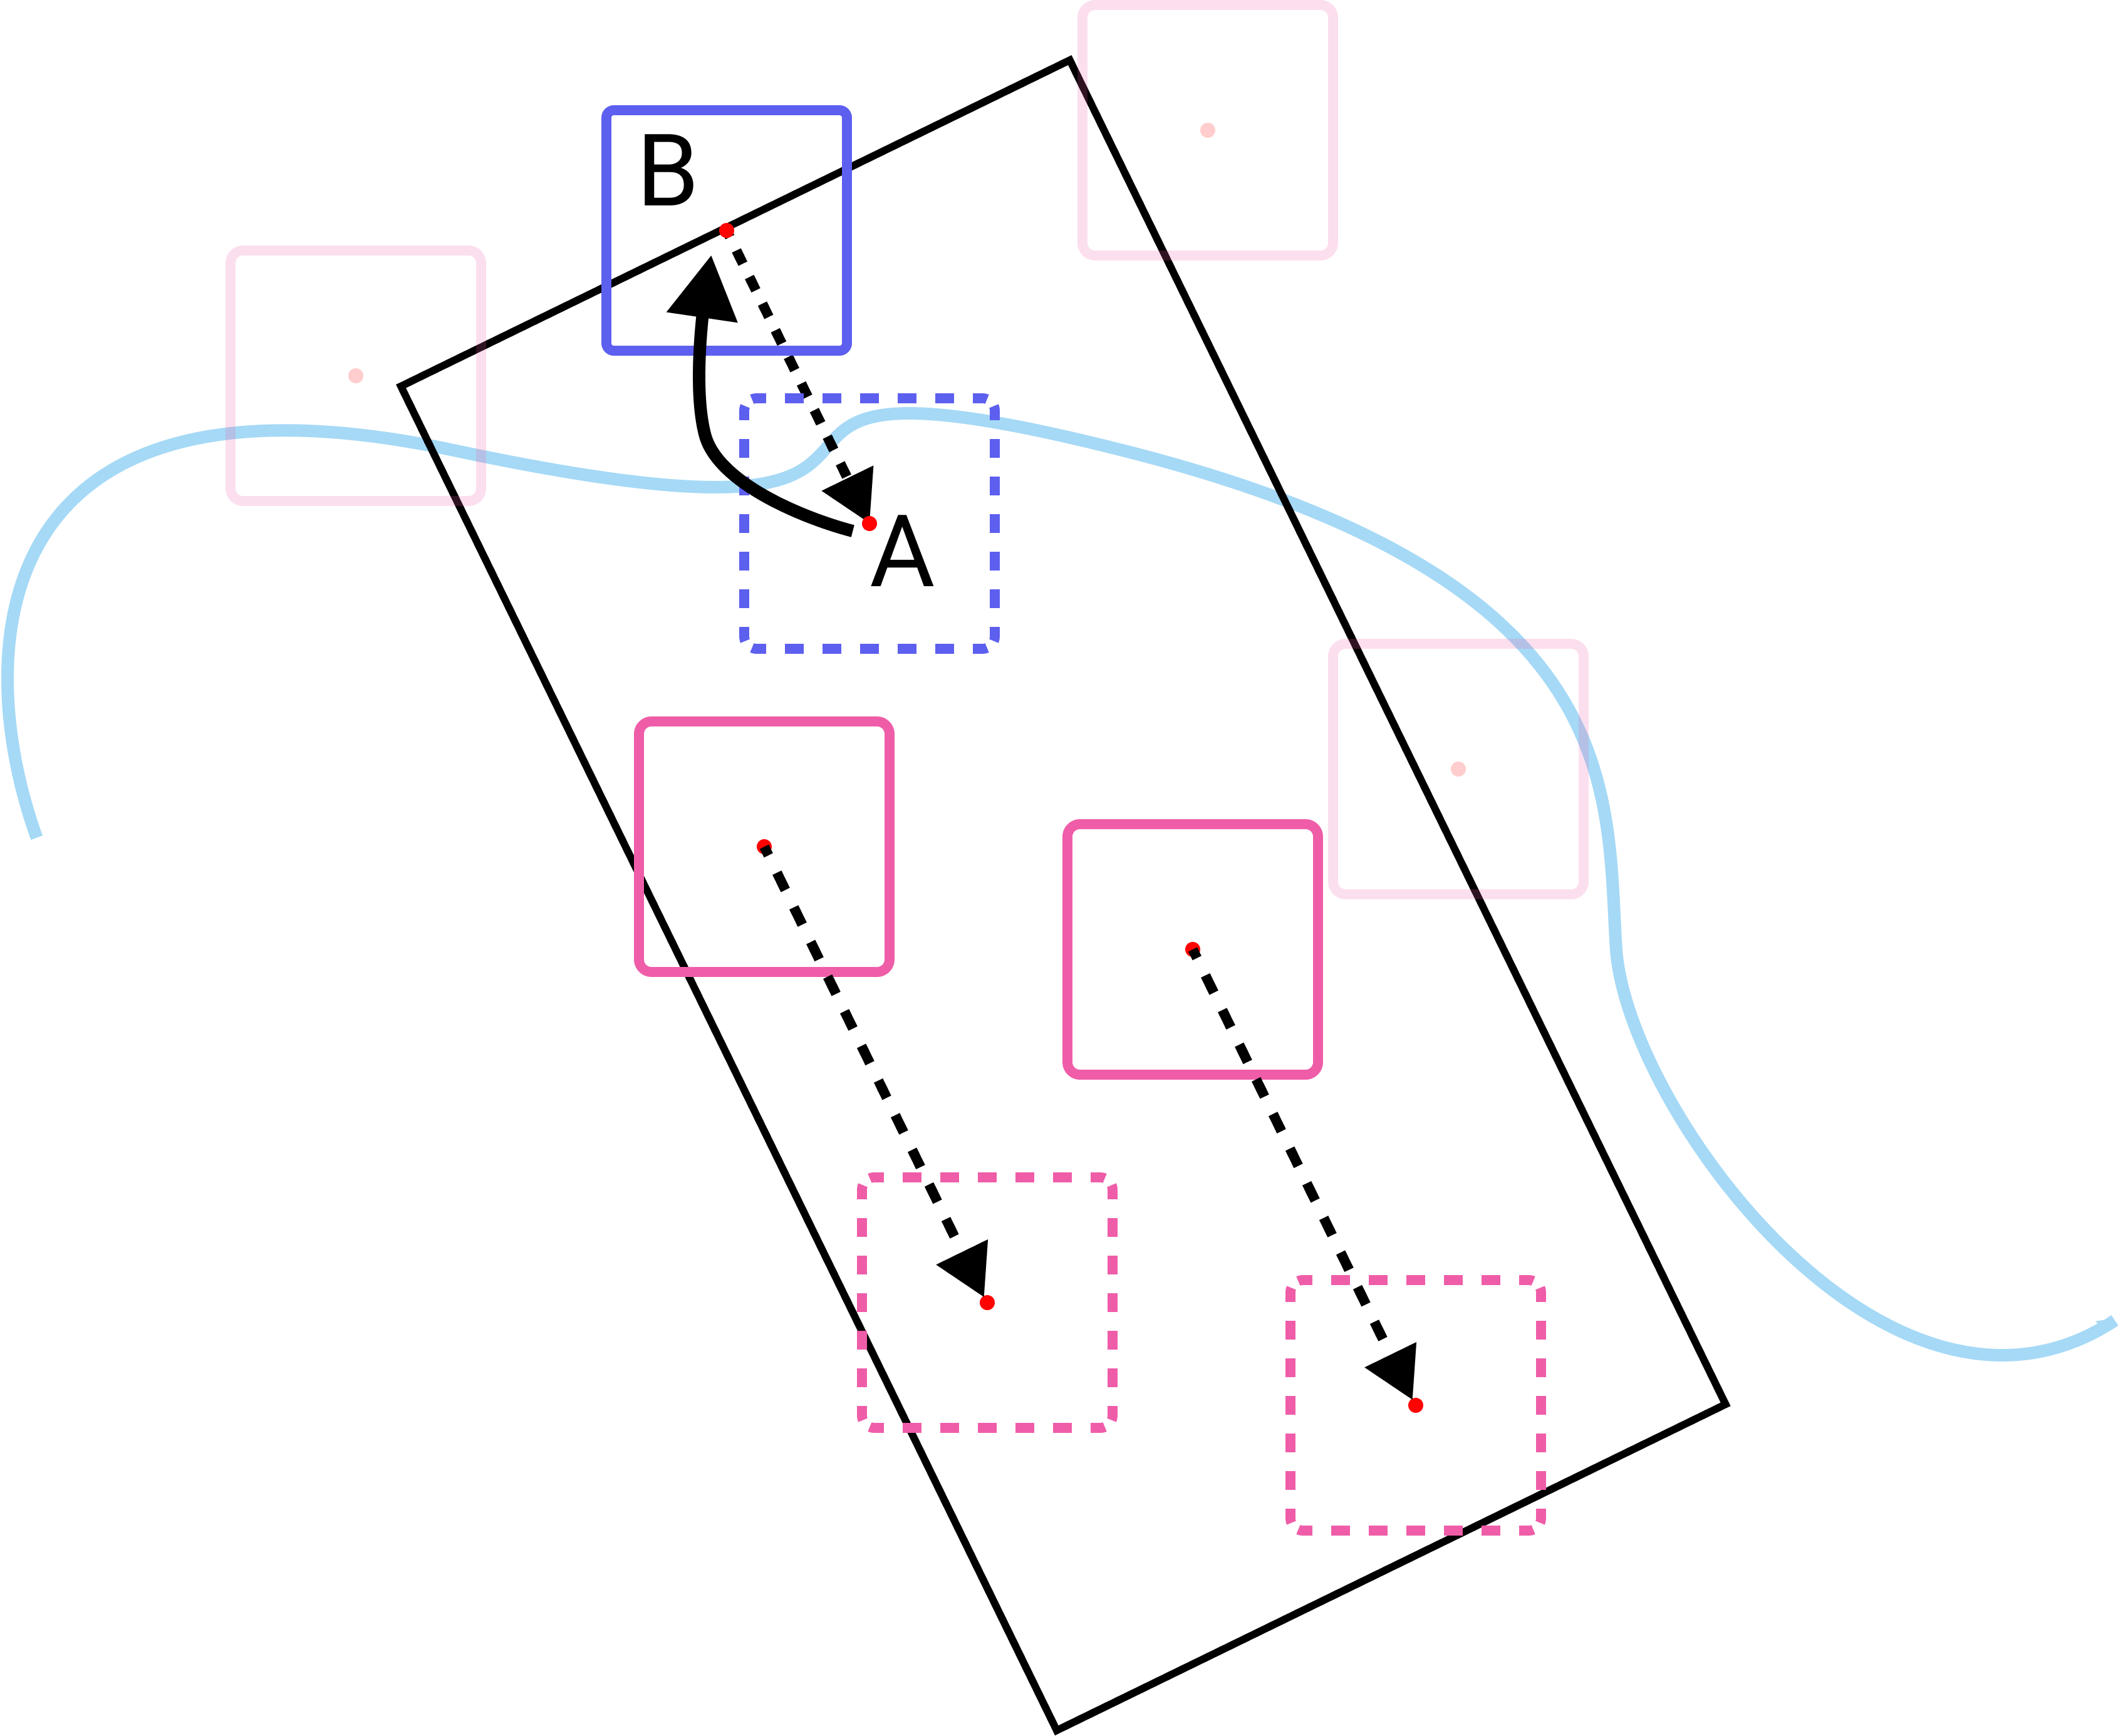
\includegraphics[width=\columnwidth]{figure/corridor.png}
    \caption{When a stalemate occurs, a corridor (black rectangular) is derived based on the current (A) and previous (B) positions of the node that crossed a river, as described in \algoref{alg:derive corridor}. All nodes within the corridor are moved by $ \mathcal{D} $ in the direction of $ \vec{BA} $. }
    \label{fig:corridor}
\end{figure}
}

% \begin{noindent}

\begin{algorithm}[tb!]
    \caption{The procedure to derive a corridor to move included nodes. We use a SVG canvas, where the point of origin (0,0) is located at the top left corner, with the x-axis extending to the right and the y-axis extending to the bottom, there is no negative axes.}\label{alg:derive corridor}
    \textbf{Variables:} \\
    $\mathcal{C}_l \gets$ the length of a corridor \\
    $\mathcal{C}_w \gets$ the width of a corridor \\
    $\mathcal{D} \gets$ the distance to move nodes within the corridor \\
    $Node_{size}\gets$ the current size of all nodes \\
    \begin{algorithmic}[1]
        \Procedure{DeriveCorridor}{$ Node, Node_{old} $}
        \State MoveNode ($ Node $)

        \State $ \Delta x \gets Node.x - Node_{old}.x,~ \Delta y \gets Node.y - Node_{old}.y $

        \State $ slope \gets \frac{\Delta x}{\Delta y}$

        \State $ pLine = $ \Call{DerivePoint}{$ \frac{-1}{ slope } $, $ Node $, $ \mathcal{C}_w $}
        \State $ sideLine_1 = $ \Call{DerivePoint}{$ slope $, $ pLine.a $, $ \mathcal{C}_l $, $ True $}
        \State $ sideLine_2 = $ \Call{DerivePoint}{$ slope $, $ pLine.b $, $ \mathcal{C}_l $, $ True $}
        \State $ corridor \gets
            \begin{bmatrix}
                pLine.a &
                pLine.b \\

                sideLine_1.a &
                sideLine_2.b \\
            \end{bmatrix} $

        \For{$ node^i $ inside $ corridor $}
            \State $ destination = $ \Call{DerivePoint}{$ \frac{-1}{ slope } $, $ node^i $, $ \mathcal{D} $}

            \State MoveNode ($ node^i, destination.b $)
        \EndFor

        \EndProcedure

        \item[]

        \Procedure{DerivePoint}{$ Slope, Point, Length, IsSideLine $}
        
        \State init. $ a $, $ b $
        \Switch{$Slope$}
            \Case{$0$}
                \If{$ IsSideLine = True $}
                    \State $ a.x \gets Point.x $
                \Else
                    \State $ a.x \gets Point.x + Length $
                \EndIf
                \State $ a.y \gets Point.y $
                \State $ b.x \gets Point.x - Length $,~$ b.y \gets Point.y $
            \EndCase
            \Case{$ \infty $ or $ -\infty $}
                \State $ a.x \gets Point.x $

                \If{$ IsSideLine = True $}
                    \State $ a.y \gets Point.y $
                \Else
                    \State $ a.y \gets Point.y + Length $
                \EndIf

                \State $ b.x \gets Point.x $,~$ b.y \gets Point.y - Length $
            \EndCase
            \Default
                \State $ dx = \sqrt{\frac{Length}{{1+Slope^2}}}$,~ $ dy = Slope \cdot dx $
                \If{$ IsSideLine = True $}
                    \State $ a.x \gets Point.x $,~$ a.y \gets Point.y $
                \Else
                    \State $ a.x \gets Point.x + dx $,~$ a.y \gets Point.y + dy $
                \EndIf

                \State $ b.x \gets Point.x - dx $,~$ b.y \gets Point.y - dy $
            \EndDefault

        \EndSwitch

        \State \Return{$ a, b $}

        \EndProcedure

    \end{algorithmic}
\end{algorithm}

%\end{noindent}